\chapter{Background Error Covariance Estimation}
\label{gen_be}

Barker, Lin

\section{Overview}

Forecast (first guess or background) error covariances are a vital input to any modern data assimilation system. They influence the analysis fit to observations and also completely define the analysis response away from observations. The latter impact is particularly important in data-sparse areas of the globe. Unlike ensemble filter data assimilation techniques (e.g. the Ensemble Adjustment Kalman Filter, the Ensemble Transform Kalman Filter), 3/4D-Var systems do not implicitly evolve forecast error covariances in real-time. Instead, climatologic statistics are typically estimated offline, and tuned to represent forecast errors for particular applications. This document describes the generation and tuning of forecast error covariances for the WRF-Var system.

WRF-Var is a freely available community variational data assimilation system. It is used in a number of applications spanning convective to synoptic scales, tropical to polar domains, and variable observation distributions. In addition, the WRF-Var system is used to provide initial conditions for a number of forecast models in addition to WRF, e.g. MM5, the Korean Meteorological Administration's (KMA's) global spectral model, and the Taiwanese Nonhydrostatic Forecast Model (NFS). Perhaps understandably, the issue of forecast error generation for WRF-Var applications is the number 1 user question to date. For all these reasons, it is therefore vital that an accurate, portable, flexible, and efficient utility to generate and tune forecast error statistics be made available for community use. 

In the next subsection, a brief overview of the role of forecast error covariances in variational data assimilation is given. Default forecast error statistics are supplied with the WRF-Var release. These data files are made available primarily for training purposes, i.e. to permit the user to configure and test the WRF-Var/WRF system in their own application. It is important to note that the default statistics are not intended for extended testing or real-time applications of WRF-Var. For those applications, there is no substitute to creating one's own forecast error covariances with the {\it gen\_be} utility, described in subsection (\ref{gen_be_sub}). Having created domain-specific statistics, it may then be necessary to further tune both forecast and observation error statistics. A variety of algorithms are supplied with WRF-Var to perform this tuning, and documented in Chapter (\ref{diagnostics}). These tuning algorithms include both innovation vector-based approaches \citep{hollingsworth86}
and variational tuning approaches \citep{desroziers01}. Clearly, the whole process of tuning error statistics for data assimilation is rather complex. However, it has been shown in many applications, that this work is vital if one is to produce the optimal analysis.

\section{Scientific Background}

As shown in Chapter (\ref{intro}), the basic goal of any variational data assimilation system is to produce an optimal estimate of the true atmospheric state at analysis time through iterative solution of a prescribed cost-function {\it J}. The particular variational data assimilation algorithm adopted in WRF-Var is a model-space, incremental formulation of the variational problem.  In this approach, observations, previous forecasts, their errors, and physical laws are combined to produce analysis increments ${\partial \bf x^{a}}$, which are added to the first guess $x_{b}$ to provide an updated analysis.

The background (or "first guess") error covariance matrix is defined as 

\begin{equation}
{\bf B}=\overline{\epsilon \epsilon^{T}} \simeq \overline{{\bf x'}{\bf x'}^{T}},
\label{var-b}
\end{equation}

\noindent where the overbar denotes an average over time, and/or geographical area. The true background error $\epsilon$ is not known in reality, but is assumed to be statistically well represented by a model state perturbation ${\bf x'}$. In the standard NMC-method \citep{parrish92}, the perturbation ${\bf x'}$ is given by the difference between two forecasts (e.g. 24 hour minus 12 hour) verifying at the same time. Climatological estimates of background error may then be obtained by averaging such forecast differences over a period of time (e.g. one month). An alternative strategy proposed by \citep{fisher03} makes use of ensemble forecast output, defining the ${\bf x'}$ vectors as ensemble perturbations (ensemble minus ensemble mean). In either approach, the end results is the same  - an ensemble of model perturbation vectors from which estimates of background error may be derived. The new {\it gen$\_$be} code has been designed to work with either forecast difference, or ensemble-based perturbations.

In model-space variational data assimilation systems, the background error covariances are specified not in model space ${\bf x'}$, but in a control variable space ${\bf v}$, related to the model variables (e.g. wind components, temperature, humidity, and surface pressure) via a control variable transform U defined by

\begin{equation}
{\bf x'} = {\rm U}{\bf v}= {\rm U}_{p} {\rm U}_{v} {\rm U}_{h}{\bf v}.
\label{var-cv}
\end{equation}

where the breakdown into components of U represents transformations of variable (p), and vertical (v) and horizontal (h) components of spatial error covariances. The transform (\ref{var-cv}), and its adjoint are required in the WRF-Var code, and will be dsecribed in more detail in Chapter (\ref{be_modeling}). In contrast, the gen\_be code performs the inverse transform

\begin{equation}
{\bf v} = {\rm U}^{-1}{\bf x'}= {\rm U}^{-1}_{h} {\rm U}^{-1}_{v} {\rm U}^{-1}_{p} {\bf x'}.
\label{var-cv-inv}
\end{equation}
in order to accumulate statistics for each component of the control vector $\bf v$. The detailed procedure for performing this calculation is described in the next section.


\section{WRF's Forecast Error Covariance Estimator - gen\_be}
\label{gen_be_sub}

The background error covariance generation code gen\_be is designed to take input from a variety of regional/global models (e.g. WRF, MM5, KMA global model, etc.), and process it in order to provide error covariance statistics. Note only the first stage (stage0) is model-specific - the output from stage0 is in a standard model-independent format. The gen\_be output forecast error statistics may be used in a variety of ways, including: i) Forecast error covariances for multi-model applications of WRF-Var, ii) Multi-model error intercomparison studies, iii) Studying multivariate correlations within ensemble prediction systems, and iv) Defining optimal control variable/balance constraints for particular applications.

The gen\_be utility comprises a number of fortran codes, as described in the following subsections. 

\subsection{gen\_be\_stage0\_wrf - Calculate perturbations of standard fields}

This stage is the only part of the process that has knowledge of the model supplying the forecast data and is specific to individual models. The purpose of this stage is to read model-specific, full field forecast data, to create model perturbations ${\bf x'}$, convert to standard perturbation fields (and metadata), and output them in a standard binary format for further processing as illustrated in Fig. 1.

Using the NMC-method, ${\bf x}'={\bf x_{T2}}-{\bf x_{T1}}$ where $T2$ and $T1$ are the forecast difference times (e.g. 48hr, 24hr for global, 24hr, 12hr for regional).  Alternatively, for an ensemble-based approach, ${\bf x_{k}}'={\bf x_{k}}-\bar{\bf x}$ where the overbar is an average over ensemble members $k=1,n_{e}$. The total number of binary files produced by stage0 is $n_{f} \times n_e$ where $n_f$ is the number of forecast times used (e.g. for 30 days with forecast every 12 hours, $n_f=60$). Using the NMC-method, $n_e=1$ (1 forecast difference per time). For ensemble-based statistics, $n_e$ is the number of ensemble members.


Fig. 1: Sketch of gen\_be's stage0 program. Model-specific (e.g. gen\_be\_stage0\_wrf for WRF) processing of full field forecast fields is performed to convert to perturbation fields of "standard" variables and relevant metadata, e.g. latitude, height, land/sea, etc.
	
Input: Model-specific forecast files.

Processing: Read forecasts, calculate ${\bf x'}$ perturbations, transform to standard perturbation fields.

Output: File containing standard fields in specific binary format, with filename e.g. \\pert.2003010112.e001 (perturbation valid at 12Z on 1 January 2003).

The standard gridpoint fields are:

\begin{itemize}\setlength{\parskip}{-4pt}
\item
 	Perturbations: Streamfunction $\psi'(i,j,k)$, velocity potential $\chi'(i,j,k)$, 
temperature $T'(i,j,k)$, relative humidity $r'(i,j,k)$, surface pressure $p_s'(i,j)$.

\item
 	Full-fields: height $z(i,j,k)$, latitude $\phi(i,j)$. (These are required for the 
production of background error statistics stored in terms of physics variables, 
rather than tied to a specific grid. This flexibility is included in {\it gen$\_$be} through a 
namelist option to define the bins over which data is averaged in a variety of ways 
(e.g., latitude height, grid points). Land-sea and orographic effects may also be 
represented in this way.
\end{itemize}

The calculation of streamfunction and velocity potential from input $u$ and $v$ fields is performed via a Fast Fourier Transform (FFT) decomposition of computed vorticity and divergence fields. Each model has it's own stage0 (only that for WRF - gen\_be\_stage0\_wrf is supported at present) which outputs a common format so that the remaining stages below are the same for all model data.


\subsection{gen\_be\_stage1 - Remove Mean}



This stage simply reads the perturbation fields output by stage0 and removes the time/bin mean from each standard field and level. The zero-mean fields are output to separate directories/files for each variable, date and member (e.g. psi/2003010112.psi.e001 contains the 3D psi field with mean removed).

Input: Perturbation fields (output of stage 0)

Processing: Remove mean for each variable/level.

Output: Standard fields: $z(i,j,k)$, $\phi(i,j)$, $\psi'(i,j,k)$, $\chi'(i,j,k)$, 
$T'(i,j,k)$, $r'(i,j,k)$, $p_s'(i,j)$.

\subsection{gen\_be\_stage2 - Calculate balance regressions coefficients}

The standard control variables (i.e. those variable for which we assume cross-correlations are zero) in WRF-Var are streamfunction, "pseudo" relative humidity, and the unbalanced components of velocity potential, temperature, and surface pressure.

The unbalanced control variables are defined as the difference between full and balanced (or correlated) components of the field. In this stage of the calculation of background errors, the balanced component of particular fields is modeled via a regression analysis of the field using specified predictor fields (e.g. streamfunction). (see \citet{wu02} for further details). The resulting regression coefficients are output for use in WRF-Var's ${\rm U}_p$ transform, and are also used in gen\_be\_stage2a (see below). Currently, three regression analyses are performed resulting in three sets of regression coefficients (note: drop the perturbation notation from now on for clarity):


\begin{itemize}\setlength{\parskip}{-4pt}
\item   Velocity potential/streamfunction regression: $\chi_b=c\psi$;
\item	Temperature/streamfunction regression: $T_{b,k1}=\sum_{k2}G_{k1,k2}\psi_{k2}$; and
\item	Surface pressure/streamfunction regression: $p_{sb}=\sum{k}W_{k}\psi_{k}$.
\end{itemize}

Data is read from all $n_f \times n_e$ files and sorted into bins defined via the namelist option {\it bin$\_$type}. Regression coefficients $G(k1,k2)$ and $W(k)$ are computed individually for each bin ({\it bin$\_$type}=1 is used here, representing latitudinal dependence) in order to allow representation of differences between e.g. polar, mid-latitude, and tropical dynamical and physical processes. In addition, the scalar coefficient $c$ used to estimate velocity potential errors from those of streamfunction is calculated as a function of height to represent e.g. the impact of boundary-layer physics. Latitudinal /height smoothing of the resulting coefficients may be optionally performed to avoid artificial discontinuities at the edges of latitude/height boxes.

In summary, gen\_be\_stage2 proceeds as follows:

Input: Standard fields (output of stage 1).

Processing: Regression analysis to determine multivariate correlations between perturbation fields.

Output: Regression coefficients $c$, $W$, $G$.


\subsection{gen\_be\_stage2a - Calculate unbalanced control variable fields}

Having computed regression coefficients, the unbalanced components of the fields are 
calculated as $\chi_u=\chi-c\psi$, $T_{u,k1}=T_{k1}-\sum_{k2}G_{k1,k2}\psi_{k2}$, 
and $p_{su}=p_s - \sum_{k} W_{k}\psi_{k}$. These fields are output for the 
subsequent calculation of the spatial covariances as described below.

Input: Standard fields (output of stage 1) and regression coefficients (output of stage 2).

Processing: Compute unbalanced components of selected fields.

Output: Unbalanced fields $\chi_u$,  $T_u$, and $p_{su}$.


\subsection{gen\_be\_stage3 - Eigenvectors/values of Vertical Error Covariances}

The gen\_be\_stage3 program calculates the statistics required for the vertical component of the control variable transform of WRF-Var. This involves the projection of 3D fields on model-levels onto empirical orthogonal functions (EOFs) of the vertical component of background error covariances \citep{barker04}.


The {\it gen$\_$be} code calculates both domain-averaged and local
values of the vertical component of the background error covariance
matrix. The definition of local again depends on the value of the
namelist variable bin$\_$type chosen. For example, for bin$\_$type=1,
a $kz \times kz$ (where $kz$ is the number of vertical levels) vertical
component of $\bf B$ is produced at every latitude (data is averaged
over time and longitude) for each control variable. Eigendecomposition
of the resulting climatological vertical error covariances ${\bf
B}={\bf E}{\Lambda}{\bf E}^{T}$ results in both domain-averaged and
local eigenvectors $\bf E$ and eigenvalues $\Lambda$. Both sets of
statistics are included in the dataset supplied to WRF-Var, allowing
the choice between homogeneous (domain-averaged) or local
(inhomogeneous) background error variances and vertical correlations
to be chosen at run time \citep{barker04}.

Having calculated and stored eigenvectors and eigenvalues, the final
part of {\it gen$\_$be$\_$stage3} is to project the entire sequence of
3D control variable fields into EOF space ${\bf v_v}=U_{v}^{-1}{\bf
v_p}=\Lambda^{-1/2}{\bf E}^{T} {\bf v_p}$.

Input: 3D (i,j,k) control variable fields: $\psi$, $\chi_u$,  $T_u$, and $r$ (output from stage 1 and 2a).

Processing: For each variable: compute vertical component of ${\bf B}$, perform eigenvector decomposition, and compute projections of fields onto eigenvectors.

Output: Eigenvectors $\bf E$, eigenvalues $\Lambda$, and projected 3D (i,j,m) control variable fields:  $\psi$, $\chi_u$,  $T_u$, and $r$ for calculation of horizontal correlations.


\subsection{gen\_be\_stage4 - Horizontal Error Correlations}

The last aspect of the climatological component of background error covariance data required for WRF-Var are the horizontal error correlations, the representation of which forms the largest difference between running WRF-Var in regional and global mode (it is however, still a fairly local change).

In global applications (gen\_be\_stage4\_global). a spectral decomposition of the grid-point data is performed, and power spectra computed for each variable and vertical mode. Details of the spectral technique used to project gridpoint fields to spectral modes are given in Appendix B together with a description of the power spectra computed from the spectral modes.

In regional applications (gen\_be\_stage4\_regional), a recursive filter is used to provide the horizontal correlations (\citet{barker04}). The error covariance inputs to the recursive filter is a correlation lengthscale (provided by gen\_be\_stage4\_regional), and a WRF-Var namelist parameters to define the correlations shape (the number of passes through the recursive filter).  The calculation of horizontal lengthscales in gen\_be\_stage4\_regional is described in section 8c of (\citet{barker04}). Note: This is the most expensive part of the entire gen\_be process.

Input: Projected 3D (i,j,m) control variable fields: $\psi$, $\chi_u$,  $T_u$, and $r$, and $p_{su}$(i,j). (output from stage 3 and 2a)

Processing (regional): Perform linear regression of horizontal correlations to calculate recursive filter lengthscales (see \citet{barker04}).

Processing (global): Perform horizontal spectral decomposition, and compute power spectra for each field/mode (see Appendix B).

Output (regional): Recursive filter lengthscales for each control variable, vertical mode.

Output (global): Power spectra for each control variable, vertical mode.


\subsection{gen\_be\_diags - Generate gen\_be.dat to be used in WRF-Var}

The gen\_be\_diags program simply gathers information from gen\_be\_stage2-4 output and writes out a file named gen\_be.dat which is one of the required input files when running WRF-Var.

Input:
\begin{itemize}\setlength{\parskip}{-4pt}
\item Regression coefficients $c$, $W$, $G$. (output of stage 2)
\item Eigenvectors $\bf E$, eigenvalues $\Lambda$. (output of stage 3)
\item Recursive filter lengthscales. (output of stage 4 regional) or Power spectra. (output of stage 4 global)
\end{itemize}

Output: A binary-format gen\_be.dat to be used in WRF-Var.


\section{Example Results from an Application of gen\_be}

Background error statistics calculated with NMC-method (24-hour and 12-hour forecast difference) from a low-resolution (200km) CONUS domain is shown in the figure below. The data period is one month in January 2003.

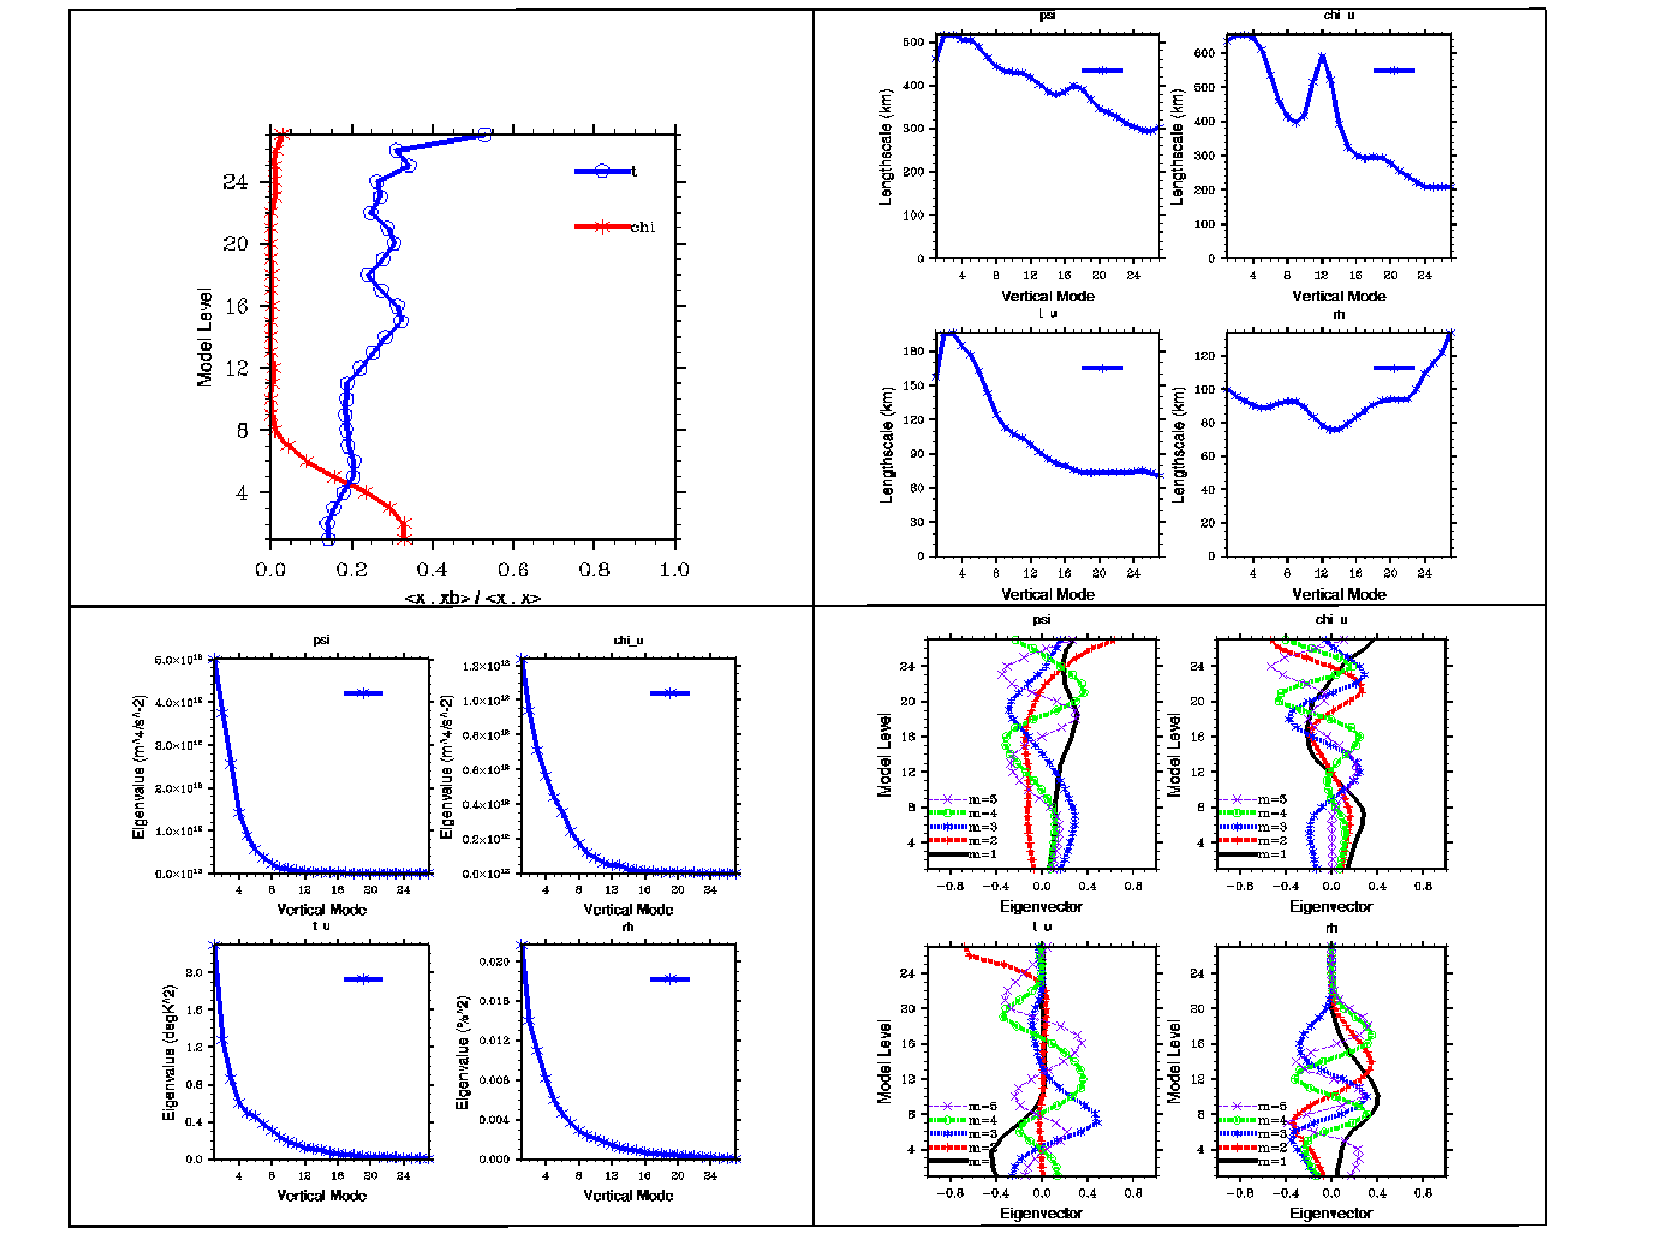
\includegraphics[width=7.0in]{figures/gen_be_results.pdf}

NCL scripts for plotting gen\_be results are included in the WRF-Var system in the directory graphics/ncl/gen\_be. The ASCII format input data required by the NCL scripts are generated using programs gen\_be\_diags\_read, gen\_be\_cov2d, and gen\_be\_cov3d in the gen\_be utility.

